\section*{Result}\label{ch:ch4label}

Learing rate 0.1 is used for a texture optimization (Cornell box) and 0.01 is used for joint optimization (Bunny)

\subsection*{Laplacian smooth version}

\subsubsection{A texture optimization}

For the comparision, MSE is estimated under the equal iterations.
currently, due to the naive implementation (3 nested for loop paralleled by only 32 threading), it is not possible to evaluate equal time comparsions. It takes eta 30 sec to compute the form $(I+\lambda)^{-1}$ under the 512x512 resolution texture every iterations. 

As shown in the figure\ref{fig:a-texture-comparision-laplacian} and table\ref{table:a-texture-comparision-laplacian}, the result indicates the faster convergence speed at the same iterations.

\begin{figure}[!h]
    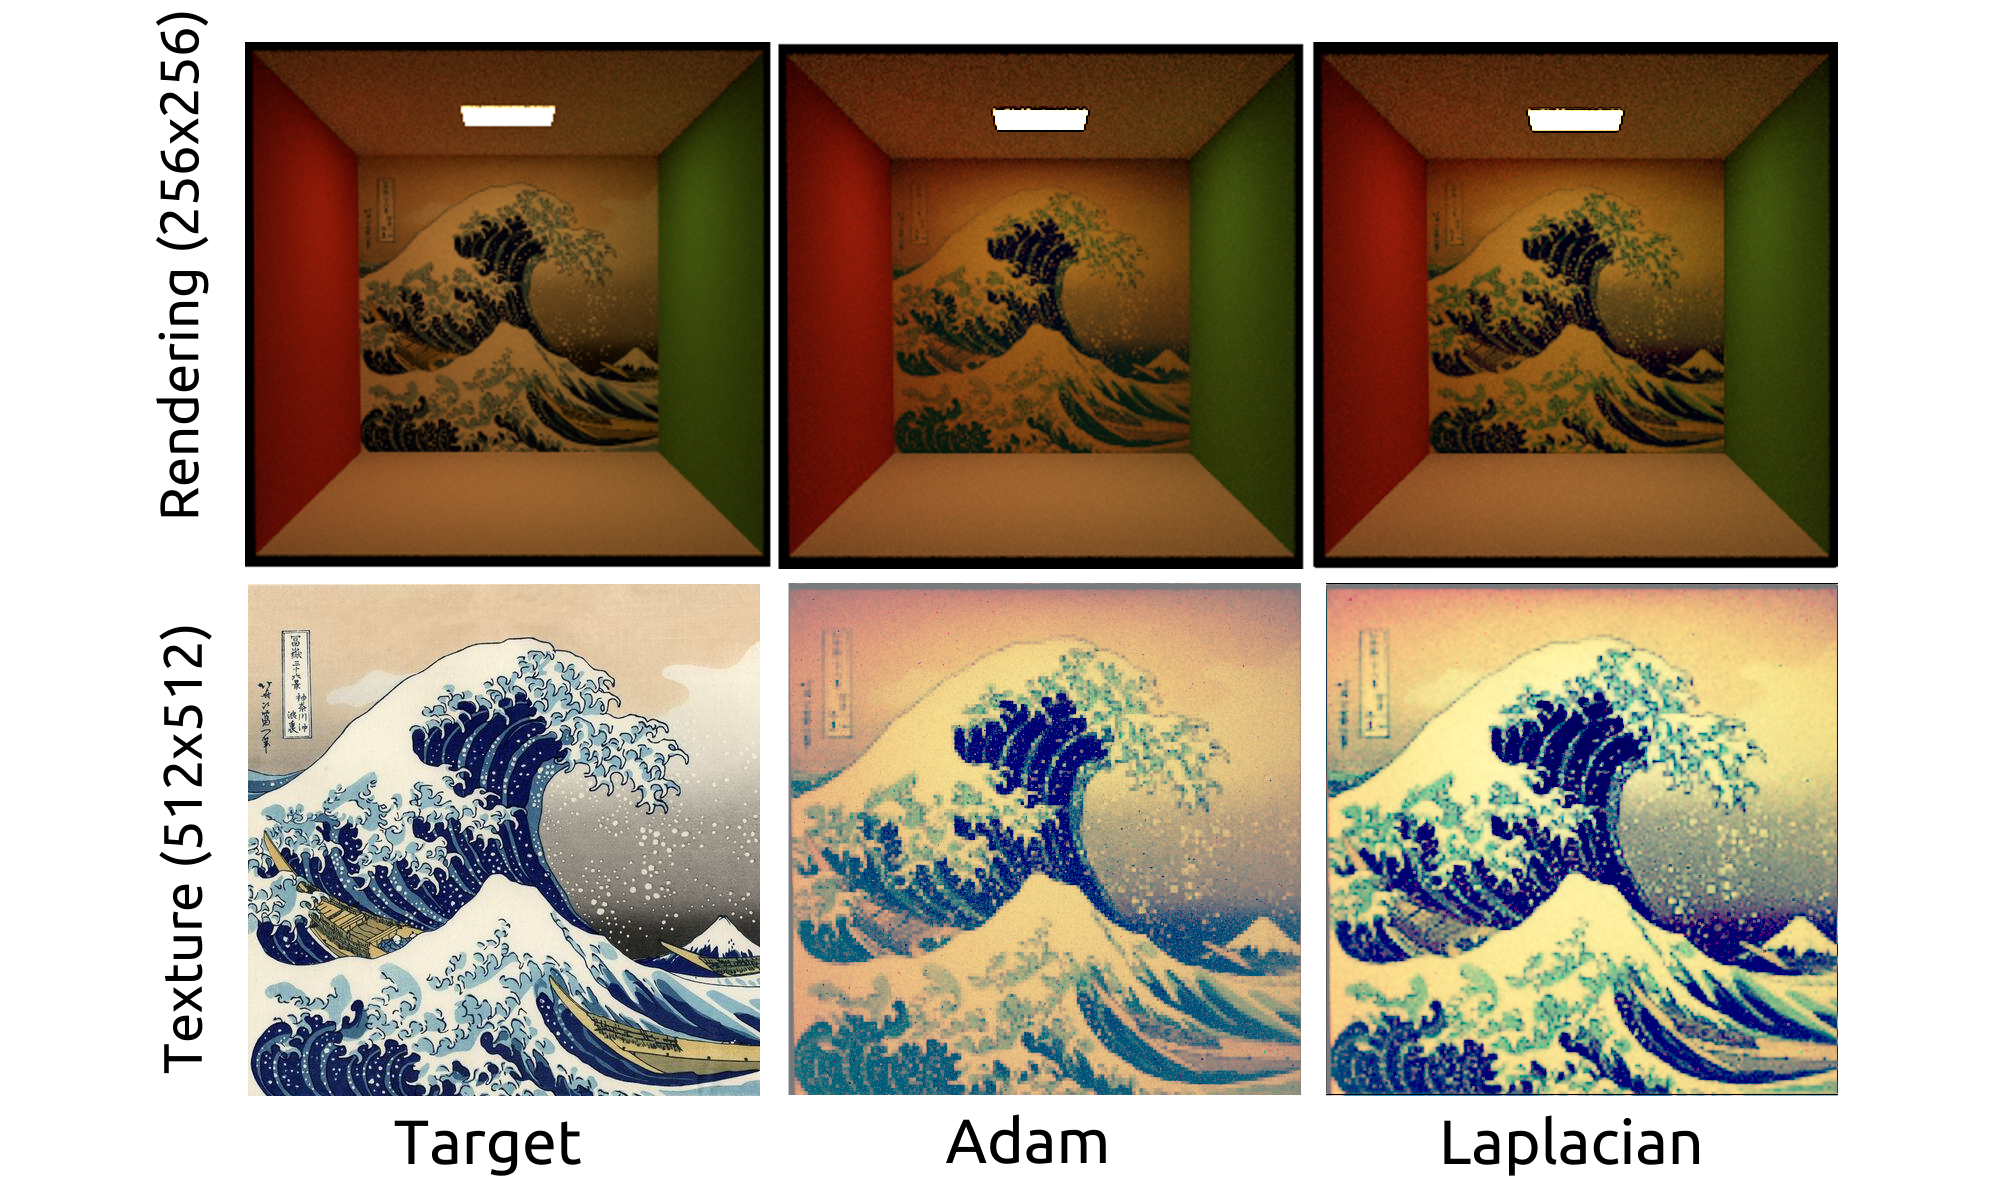
\includegraphics[width=\textwidth]{figures/result-1.png}
    \caption{comparision of a large steps texture optimization}
    \label{fig:a-texture-comparision-laplacian}
\end{figure}

\begin{table}[!h]
	\centering
	\resizebox{\textwidth}{!}{
	\begin{tabular}{ | c | c | c | c | c | c | c | c | c | c | c | c } \hline
		iter      & 1      & 2      & 3      & 4      & 5      & 6      & 7      & 8      & 9      & 10     \\\hline
		Adam      & 0.1433 & 0.1229 & 0.1060 & 0.0920 & 0.0808 & 0.0718 & 0.0647 & 0.0593 & 0.0554 & 0.0525 \\ \hline  
		Laplacian & 0.1433 & 0.1168 & 0.09453 & 0.0767 & 0.0627 & 0.0526 & 0.0456 & 0.0414 & 0.0394 & 0.0386 \\ \hline
	\end{tabular}}
	\caption{comparision of a large steps texture optimization}
	\label{table:a-texture-comparision-laplacian}
\end{table}

\subsubsection{Joint optimization for two texture (Albedo texture and Environment map)}

However, in the joint optimization case, 

Every iteration, generate artifacts image result only on the environment map. For the analysis, when we target to optimize , this indicates that the assumption to apply large steps technique to environment map is broken, neighborhood from the kernel in enviroment map

\begin{figure}[!h]
    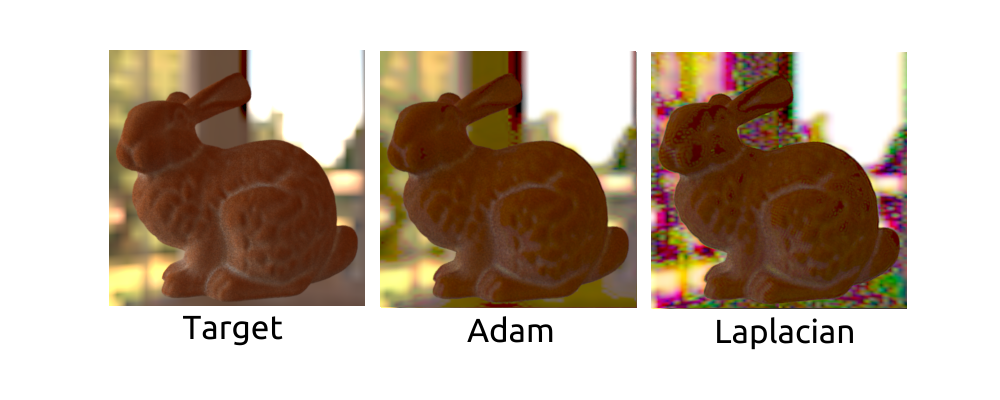
\includegraphics[width=\textwidth]{figures/result-2.png}
    \caption{comparision of a large steps joint texture optimization}
    \label{fig:a-texture-comparision-joint}
\end{figure}

\begin{figure}[!h]
    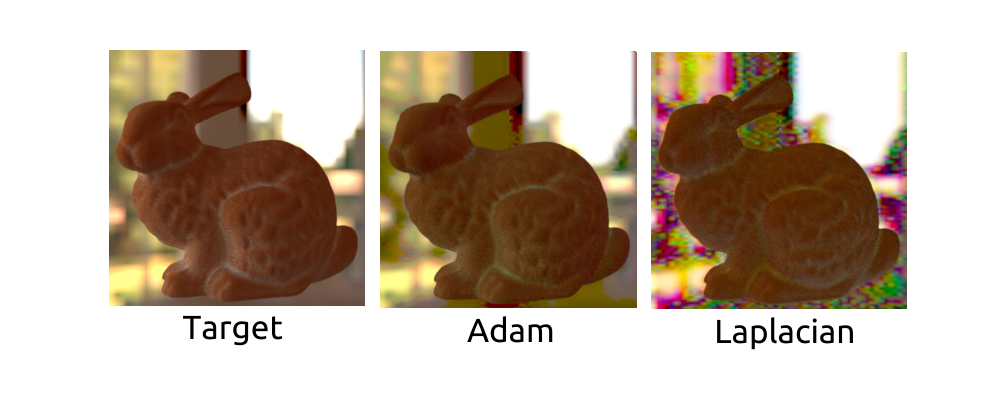
\includegraphics[width=\textwidth]{figures/result-2-1.png}
    \caption{comparision of a texture optimization result}
    \label{fig:a-texture-comparision}
\end{figure}

\subsection*{Biased version: just gaussian filtering}

Laplacian smooth gradient descent can be known propertices of original target parameters. 
biased version

\begin{figure}[!h]
    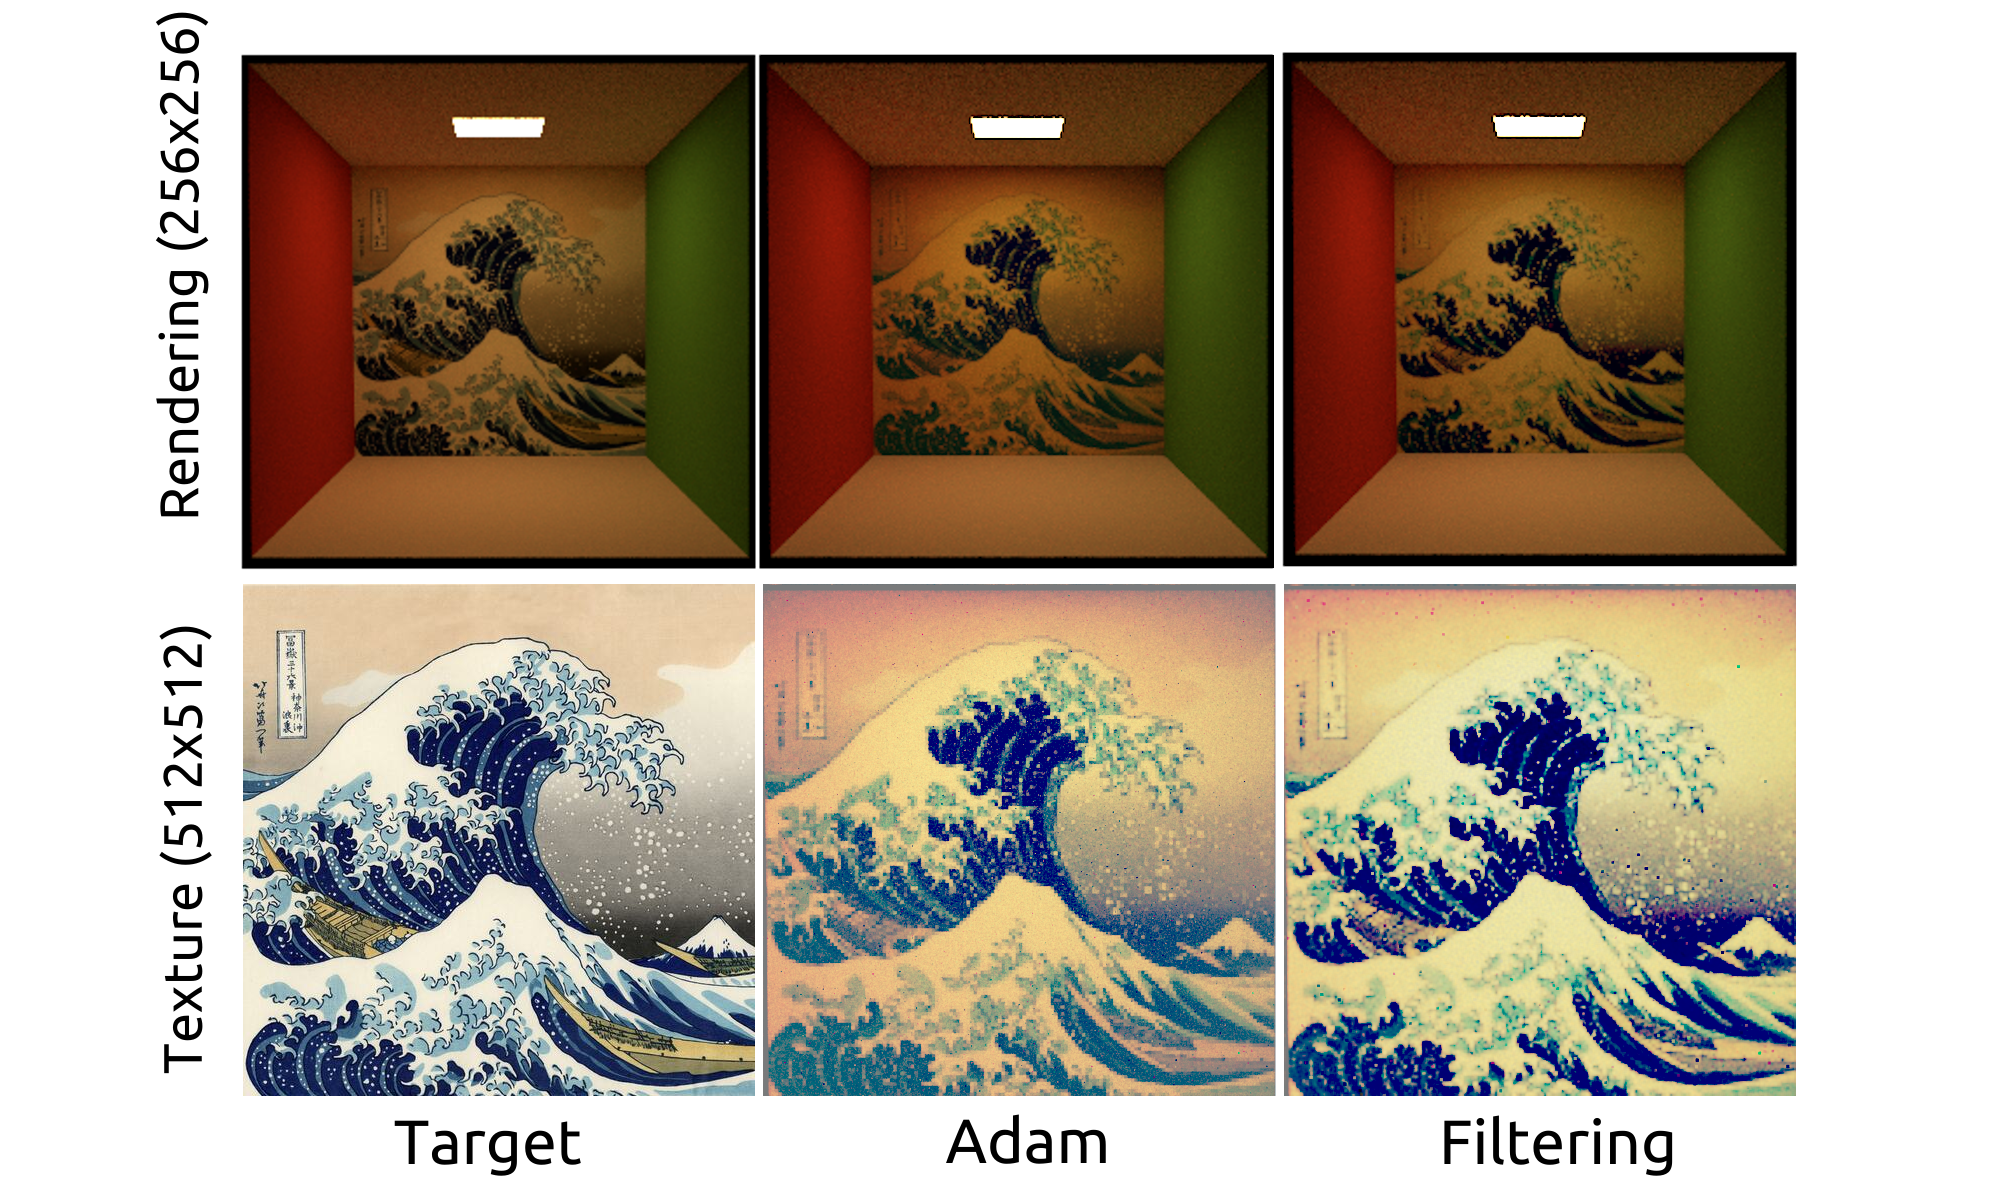
\includegraphics[width=\textwidth]{figures/result-3.png}
    \caption{comparision of a texture optimization result}
    \label{fig:a-texture-comparision}
\end{figure}


\begin{figure}[!h]
    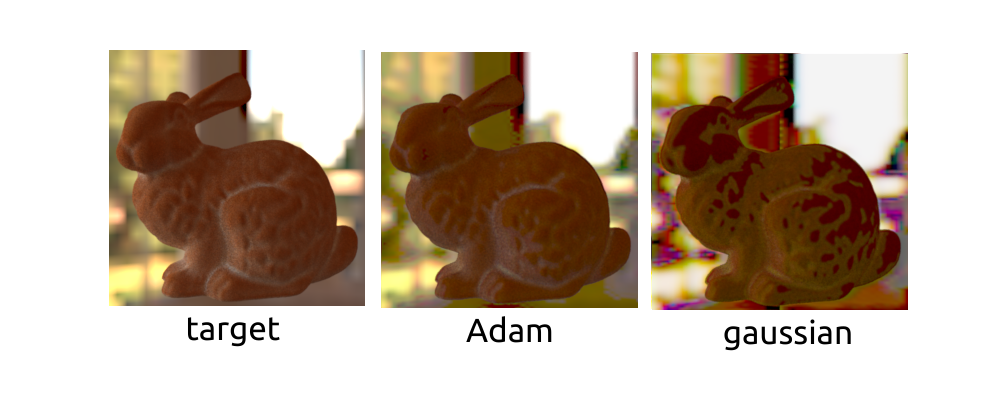
\includegraphics[width=\textwidth]{figures/result-4.png}
    \caption{comparision of a texture optimization result}
    \label{fig:a-texture-comparision}
\end{figure}

